\documentclass[a4paper,11pt]{article}

%%%%%%%%%%%%%%%%%%%%%%%%%%%%%%%%%%%%%%%%%%%%%%%%%%%%%%%%%%%%%%%%%%%%%%%%
% Paquetes utilizados
%%%%%%%%%%%%%%%%%%%%%%%%%%%%%%%%%%%%%%%%%%%%%%%%%%%%%%%%%%%%%%%%%%%%%%%%

% Gráficos complejos
\usepackage{graphicx}
\usepackage{caption}
\usepackage{subcaption}
\usepackage{placeins}

% Soporte para el lenguaje español
\usepackage{textcomp}
\usepackage[utf8]{inputenc}
\usepackage[T1]{fontenc}
\DeclareUnicodeCharacter{B0}{\textdegree}
\usepackage[spanish]{babel}

% Código fuente embebido
\usepackage{listings}
\usepackage{courier}

% PDFs embebidos para el apéndice
\usepackage{pdfpages}

% Matemáticos
\usepackage{amssymb,amsmath}

% Tablas complejas
\usepackage{multirow}

% Formato de párrafo
\setlength{\parskip}{1ex plus 0.5ex minus 0.2ex}

% Formato de listados de código
\lstset{
  basicstyle=\footnotesize\ttfamily,
  numbers=left,
  numberstyle=\tiny,
  numbersep=5pt,
  tabsize=2,
  extendedchars=true,
  breaklines=true,
  frame=t,
  showspaces=false,
  showtabs=false,
  showstringspaces=false,
  language=Java,
  caption=\lstname,
  captionpos=t
}

%%%%%%%%%%%%%%%%%%%%%%%%%%%%%%%%%%%%%%%%%%%%%%%%%%%%%%%%%%%%%%%%%%%%%%%%
% Título
%%%%%%%%%%%%%%%%%%%%%%%%%%%%%%%%%%%%%%%%%%%%%%%%%%%%%%%%%%%%%%%%%%%%%%%%

% Título principal del documento.
\title{\textbf{Trabajo Práctico Individual N°1}}

% Información sobre los autores.
\author{
  Andrés Gastón Arana(and2arana@gmail.com), \textit{P. 86.203}     \\
  \normalsize{1er. Cuatrimestre de 2013}                           \\
  \normalsize{75.10 - Técnicas de Diseño}                          \\
  \normalsize{Facultad de Ingeniería, Universidad de Buenos Aires}
}
\date{}

%%%%%%%%%%%%%%%%%%%%%%%%%%%%%%%%%%%%%%%%%%%%%%%%%%%%%%%%%%%%%%%%%%%%%%%%
% Documento
%%%%%%%%%%%%%%%%%%%%%%%%%%%%%%%%%%%%%%%%%%%%%%%%%%%%%%%%%%%%%%%%%%%%%%%%

\begin{document}

% ----------------------------------------------------------------------
% Top matter
% ----------------------------------------------------------------------
\thispagestyle{empty}
\maketitle

\begin{abstract}

  Este informe sumariza el desarrollo del trabajo práctico de la materia
  Técnicas de Diseño (75.10) dictada en el primer cuatrimestre de 2013 en la
  Facultad de Ingeniería de la Universidad de Buenos Aires. El mismo consiste
  en el refactoring de una aplicación existente para posteriormente añadir
  funcionalidad sobre la misma, utilizando siempre técnicas de testing
  automatizado para asegurar el correcto comportamiento del software.

\end{abstract}

\clearpage

% ----------------------------------------------------------------------
% Tabla de contenidos
% ----------------------------------------------------------------------
\tableofcontents
\clearpage


% ----------------------------------------------------------------------
% Desarrollo
% ----------------------------------------------------------------------
\part{Desarrollo}

\section{Análisis del diseño original} \label{sec:analisis}

El diseño original de la aplicación consistía en apenas 2 clases que
representaban varios conceptos del modelo de dominio:

\begin{enumerate}

  \item \textbf{Item} Clase que únicamente contiene los datos de un item en
    inventario.

  \item \textbf{Inventory} Clase que contiene toda la lógica de la progresión
    de calidad sobre los items contenidos en la tienda, así como la definición
    de los items propios de la misma.

\end{enumerate}

Se detectaron varios problemas con este diseño que influían negativamente en la
posibilidad de extender el programa adaptándolo a las nuevas necesidades:

\begin{enumerate}

  \item La clase \textbf{Item} es completamente anémica, limitándose a contener
    los datos de un item en inventario.

  \item La clase \textbf{Inventario} viola el principio de responsabilidad
    única, dado que es la encargada de contener los items de la tienda así como
    de llevar adelante la progresión de las calidades de los diferentes items
    en el mismo.

  \item La clase \textbf{Inventario} viola además el principio de apertura a
    extensión y clausura ante cambios, de diversas maneras. Por un lado,
    cualquier tipo de modificación en las reglas actuales de progresión de
    calidad de cualquiera de los items implica modificar el código de esta
    clase, muchas veces en varios secciones de código del único método
    responsable de realizar estos cálculos. Por otro lado, la extensión del
    software al agregar una nueva progresión implica realizar modificaciones
    similares en el mismo método.

  \item La lógica de determinación de progresiones se realiza a base de los
    nombres de los items inventariados. De esta forma, cualquier cambio en la
    manera en la que se muestran los items impacta en el procesamiento de la
    progresión de calidad. Más aún, implementar un nuevo item similar a los que
    ya existen (por ejemplo, un nuevo backstage pass) implica impactar en el
    cálculo de todos los diferentes tipos de items ya registrados.

\end{enumerate}

Debido a estas desventajas, se decidió implementar un nuevo diseño para
resolver estos problemas antes de realizar lo propio con la nueva
funcionalidad, utilizando una estrategia de refactoring con apoyo continuo en
tests automatizados para validar la funcionalidad del software. Posteriormente
se implementaron los nuevos requisitos extendiendo el diseño desarrollado.

\section{Infraestructura de desarrollo}

Primeramente se constituyó un sistema de build automatizado para poder
compilar, testear y empaquetar la aplicación de una manera sencilla, de manera
de permitir a futuros equipos de desarrollo minimizar su tiempo de setup de
ambiente, además de poder conformar un entorno de desarrollo adecuado para las
tareas de refactoring y test automatizado continuo a realizar. Para el mismo se
decidió utilizar \textbf{Gradle}, debido a su simplicidad de uso y configuración.
Debido a los requisitos de esta herramienta, se conformó la estructura de
directorios que se necesitaban para poder utilizarla, además de agregar los
archivos de configuración necesarios.

Se agregó además un archivo README.md en el root del proyecto para facilitar el
seteo inicial del ambiente.

\section{Propuesta de diseño}

En la figura \ref{fig:clases} se incluye el diagrama de clases completo de la
solución desarrollada.

\begin{figure}[h!t]
  \centering
  \includegraphics[width=1.50\textwidth, angle=90]{build/docs/uml.png}
  \caption{Diagrama de clases de la solución presentada} \label{fig:clases}
\end{figure}

\FloatBarrier

Se decidió atacar los problemas mencionados sobre el diseño anterior
identificando un nuevo concepto del dominio del problema, la \textbf{categoría}
a la que pertenece un item. Esta categoría es la que implementa las reglas de
progresión de calidad de un conjunto específico de items. Cada item pertenece a
una única categoría que define cómo se comporta al finalizar cada día, cada
categoría puede contener diversos items que se comportan de manera similar.

Para modelar este nuevo concepto, se introduce la interfase \textbf{Category},
que representa una categoría de progresión de calidad que contiene varios items
individuales que le pertenecen. Se diseño luego una jerarquía de herencia para
implementar cada una de las reglas de progresión en una especialización
particular de esta jerarquía, de manera que cada una de ellas esté aislada lo
más posible del resto. De esta forma logramos cumplir con la apertura a la
extensión y clausura ante cambios en el software.

Debido a la imposibilidad de modificar la clase \textbf{Item}, se decidió
implementar una clase \textbf{InventoriedItem} que agrega funcionalidad y
sintaxis nueva al momento de definir y trabajar con los items:

\begin{itemize}

  \item Define un constructor que acepta tipos concretos en vez de tipos
    estándar para la definición de la calidad inicial del item y su fecha de
    venta. Esto permite utilizar la sintaxis que se ejemplifica en la clase
    \textbf{Inventory}, que si bien es marginalmente menos performante es mucho
    más claro en cuanto al objetivo que cumple cada parámetro.

  \item Define métodos para modificar la calidad de un item atómicamente, con
    chequeo de condiciones de borde.

  \item Define propiedades introspectivas del estado del item, como conocer si
    un item ya superó su fecha de venta.

\end{itemize}

Una vez extraídas las diferentes responsabilidades que en el diseño original
estaban en la clase \textbf{Inventory}, esta fue modificada de manera de servir
como fachada del sistema de inventario, definiendo únicamente cuáles son los
items que se encuentran en la tienda.

\section{Análisis de la nueva propuesta}

El nuevo diseño soluciona los problemas enumerados en la sección
\ref{sec:analisis}. Cada estrategía de progresión de calidad ahora tiene su
propia clase que la implementa, de manera de que las modificaciones en una de
ellas no impactan en el resto. Además, agregar nuevas categorías (como la
implementada para el nuevo requisito del enunciado) implica únicamente agregar
una nueva clase que implemente la nueva lógica asociada, y configurar luego qué
items pertenecen a esa categoría en el inventario. Agregar nuevos items también
es mucho más simple: si la categoría ya existe, es cuestión de registrar en el
inventario al nuevo item, asociándolo a la categoría correspondiente.

Existen sin embargo algunas mejoras que se podrían realizar sobre el diseño
presentado:

\begin{enumerate}

  \item Se podría reemplazar el concepto de las categorías que disminuyen cada
    día su sell in que ahora está representado por la clase base
    \textbf{SellDueCategory} por un diseño más flexible utilizando el patrón
    \textbf{Decorator}. De esta manera, se podría definir un decorator que
    realiza la progresión del sell in, y categorías independientes que calculan
    la progresión de la calidad. Componiendo el decorador con las categorías
    como indica el patrón, se podría obtener un diseño más flexible en cuanto a
    la asignación de estos dos conceptos ortogonales.

    Este diseño no fue implementado dado que no se considera inmediata la
    necesidad de asociar diferentes categorías con este comportamiento de
    manera componible, ni tampoco se detecta la necesidad de componer diversas
    de estas estrategías simultáneamente, por lo que se considera que el diseño
    actual es suficiente.

  \item Se podría extraer la lógica de configuración de los items del
    inventario y sus categorías afuera de la clase \textbf{Inventory},
    posiblemente a un módulo que cargue dicha configuración desde un archivo
    externo o sistema de base de datos. De esta forma, se podrían agregar,
    modificar y quitar items sin tener que modificar el programa, únicamente
    cambiando la configuración de los items que se cargan en el inventario.

    Este cambio no fue implementado debido a que fue considerado fuera del
    alcance del trabajo práctico.

\end{enumerate}

\clearpage

\part{Apéndice}
\appendix

\section{Código fuente modificado}

\lstinputlisting{src/main/java/com/alexaitken/gildedrose/inventory/InventoriedItem.java}
\lstinputlisting{src/main/java/com/alexaitken/gildedrose/inventory/Inventory.java}
\lstinputlisting{src/main/java/com/alexaitken/gildedrose/inventory/Item.java}
\lstinputlisting{src/main/java/com/alexaitken/gildedrose/inventory/categories/AgedCategory.java}
\lstinputlisting{src/main/java/com/alexaitken/gildedrose/inventory/categories/BackstagePassCategory.java}
\lstinputlisting{src/main/java/com/alexaitken/gildedrose/inventory/categories/BaseCategory.java}
\lstinputlisting{src/main/java/com/alexaitken/gildedrose/inventory/categories/Category.java}
\lstinputlisting{src/main/java/com/alexaitken/gildedrose/inventory/categories/ConjuredCategory.java}
\lstinputlisting{src/main/java/com/alexaitken/gildedrose/inventory/categories/DefaultCategory.java}
\lstinputlisting{src/main/java/com/alexaitken/gildedrose/inventory/categories/LegendaryCategory.java}
\lstinputlisting{src/main/java/com/alexaitken/gildedrose/inventory/categories/SellDueCategory.java}

\FloatBarrier
\clearpage

\section{Código fuente de tests}

\lstinputlisting{src/test/java/com/alexaitken/gildedrose/inventory/BaseJUnit4Test.java}
\lstinputlisting{src/test/java/com/alexaitken/gildedrose/inventory/InventoriedItemTest.java}
\lstinputlisting{src/test/java/com/alexaitken/gildedrose/inventory/categories/AgedCategoryTest.java}
\lstinputlisting{src/test/java/com/alexaitken/gildedrose/inventory/categories/BackstagePassCategoryTest.java}
\lstinputlisting{src/test/java/com/alexaitken/gildedrose/inventory/categories/BaseCategoryTest.java}
\lstinputlisting{src/test/java/com/alexaitken/gildedrose/inventory/categories/ConjuredCategoryTest.java}
\lstinputlisting{src/test/java/com/alexaitken/gildedrose/inventory/categories/DefaultCategoryTest.java}
\lstinputlisting{src/test/java/com/alexaitken/gildedrose/inventory/categories/LegendaryCategoryTest.java}
\lstinputlisting{src/test/java/com/alexaitken/gildedrose/inventory/categories/SellDueCategoryTest.java}

\FloatBarrier
\clearpage

\section{Enunciado original}\label{sec:enunciado}
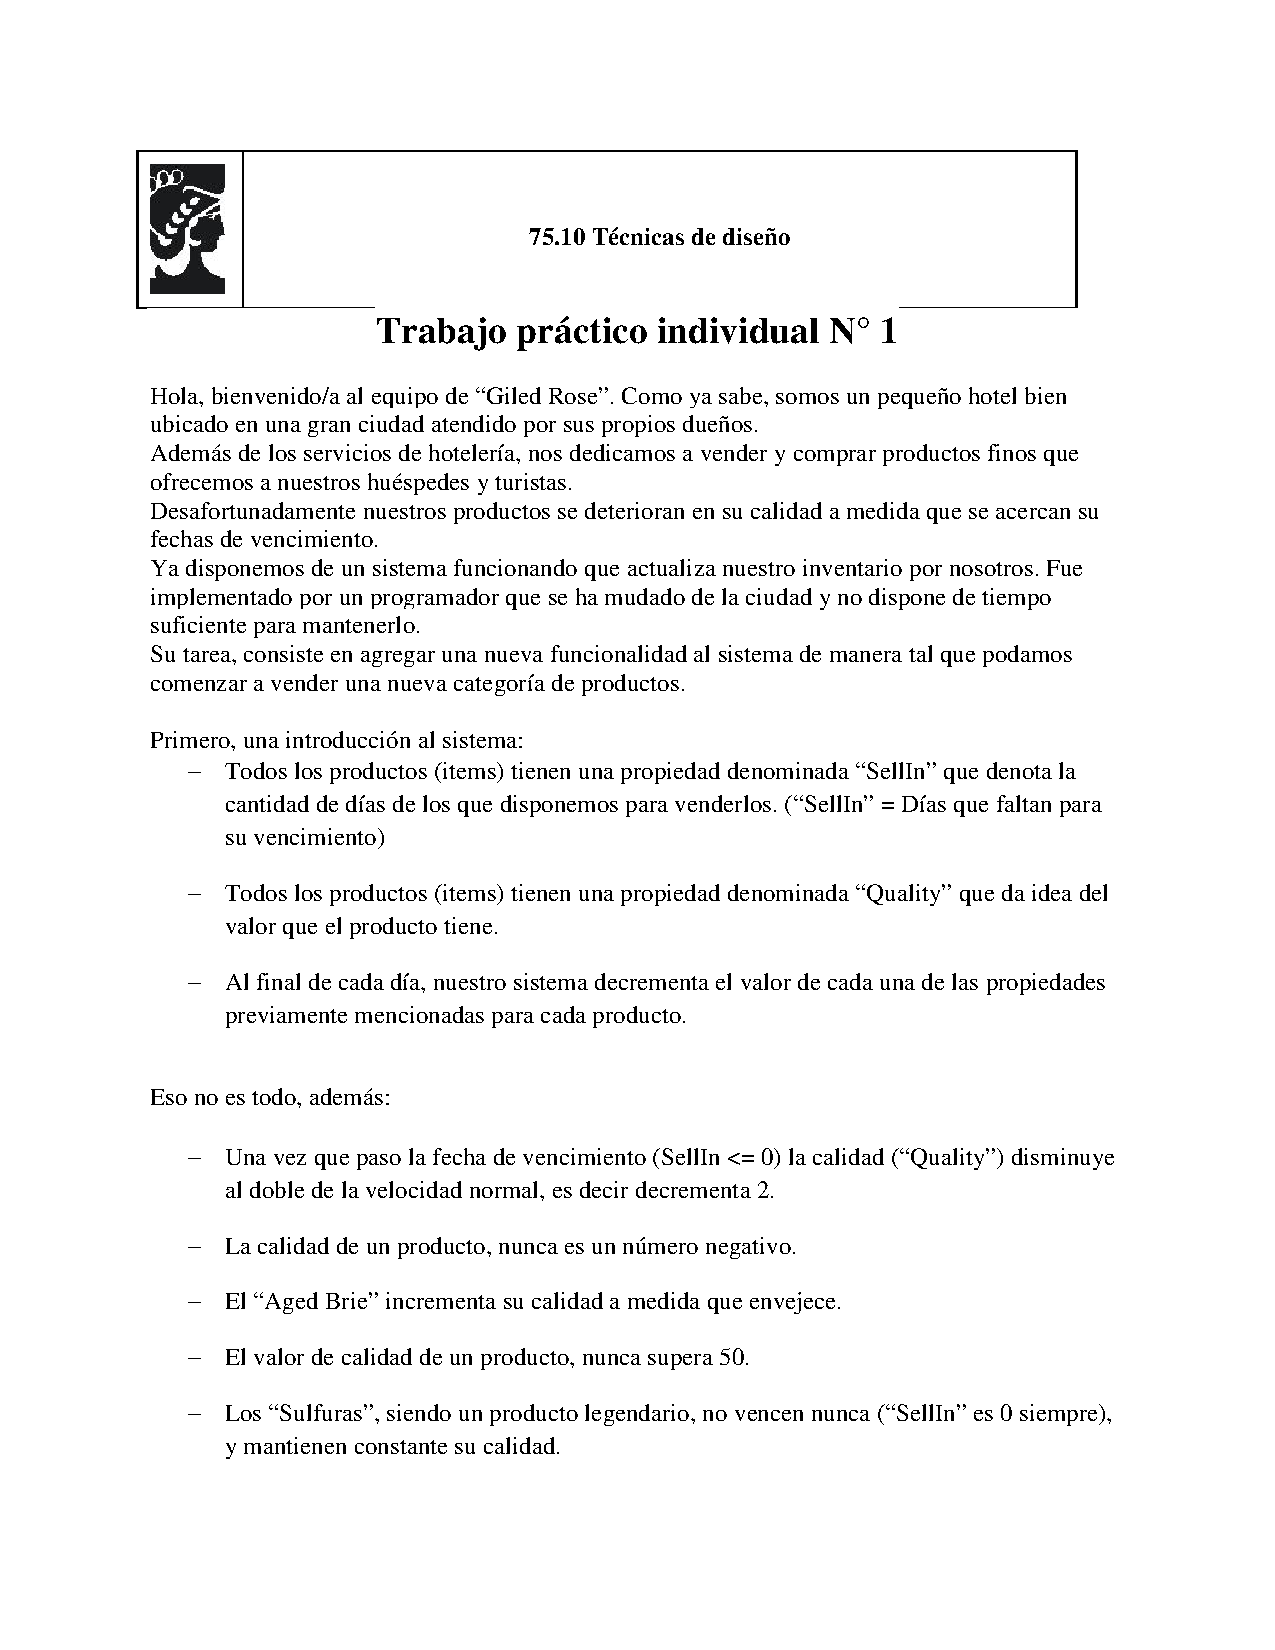
\includepdf[pages={-}, frame=true, pagecommand={}, noautoscale=true, scale=0.7]{src/docs/enunciado.pdf}

\end{document}

